\begin{figure}[t]
    \centering
    \begin{subfigure}[b]{0.3\textwidth}
        \centering
        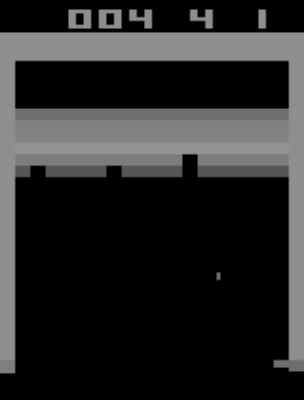
\includegraphics[width=0.62\textwidth]{figures/experiments/environments/breakout.png}
        \caption{Breakout}
        \label{fig:environment_breakout}
    \end{subfigure}
    \hfill
    \begin{subfigure}[b]{0.3\textwidth}
        \centering
        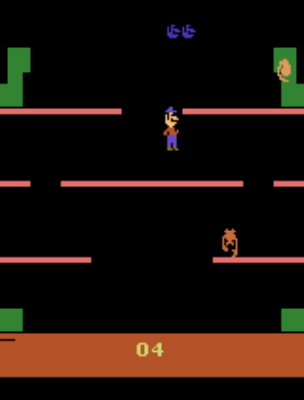
\includegraphics[width=0.62\textwidth]{figures/experiments/environments/mario_bros.png}
        \caption{Mario Bros}
        \label{fig:environment_mario_bros}
    \end{subfigure}
    \hfill
    \begin{subfigure}[b]{0.3\textwidth}
        \centering
        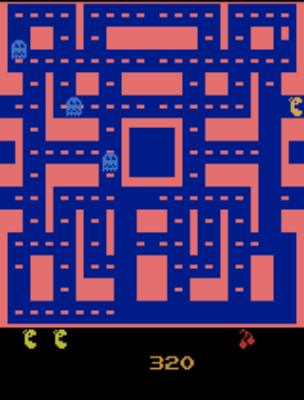
\includegraphics[width=0.62\textwidth]{figures/experiments/environments/ms_pacman.png}
        \caption{Ms.\ Pac-Man}
        \label{fig:environment_ms_pacman}
    \end{subfigure}

    \vspace{0.4cm}

    \begin{subfigure}[b]{0.3\textwidth}
        \centering
        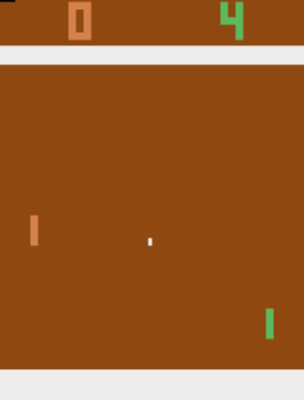
\includegraphics[width=0.62\textwidth]{figures/experiments/environments/pong.png}
        \caption{Pong}
        \label{fig:environment_pong}
    \end{subfigure}
    \hfill
    \begin{subfigure}[b]{0.3\textwidth}
        \centering
        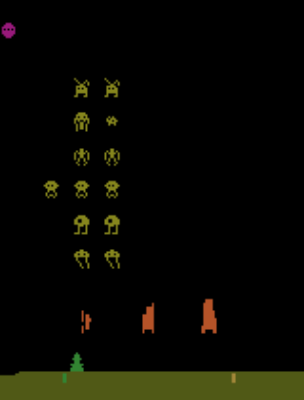
\includegraphics[width=0.62\textwidth]{figures/experiments/environments/space_invaders.png}
        \caption{Space Invaders}
        \label{fig:environment_space_invaders}
    \end{subfigure}
    \hfill
    \begin{subfigure}[b]{0.3\textwidth}
        \centering
        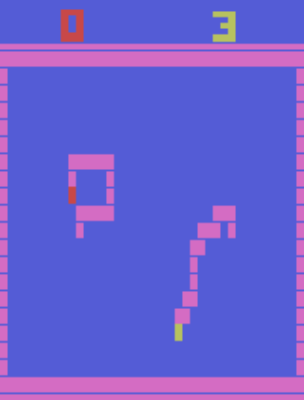
\includegraphics[width=0.62\textwidth]{figures/experiments/environments/surround.png}
        \caption{Surround}
        \label{fig:environment_surround}
    \end{subfigure}
    \caption{
        The six Atari environments used to evaluate \gls{car}, shown as rendered game frames.
        The agent does not receive these frames directly: each observation is a stack of four consecutive frames, resized to $64 \times 64$ pixels and converted to grayscale, except for Ms.\ Pac-Man, which is kept in color.
    }
    \label{fig:environments}
\end{figure}
